\setcounter{secnumdepth}{-1}
\section{Anhang A}
\setcounter{secnumdepth}{3}
\renewcommand{\thefigure}{A\arabic{figure}}
\setcounter{figure}{0}
\subsection*{Abbildungen von Frequenz�berpr�fung}
\begin{figure}[htbp] 
	\centering
	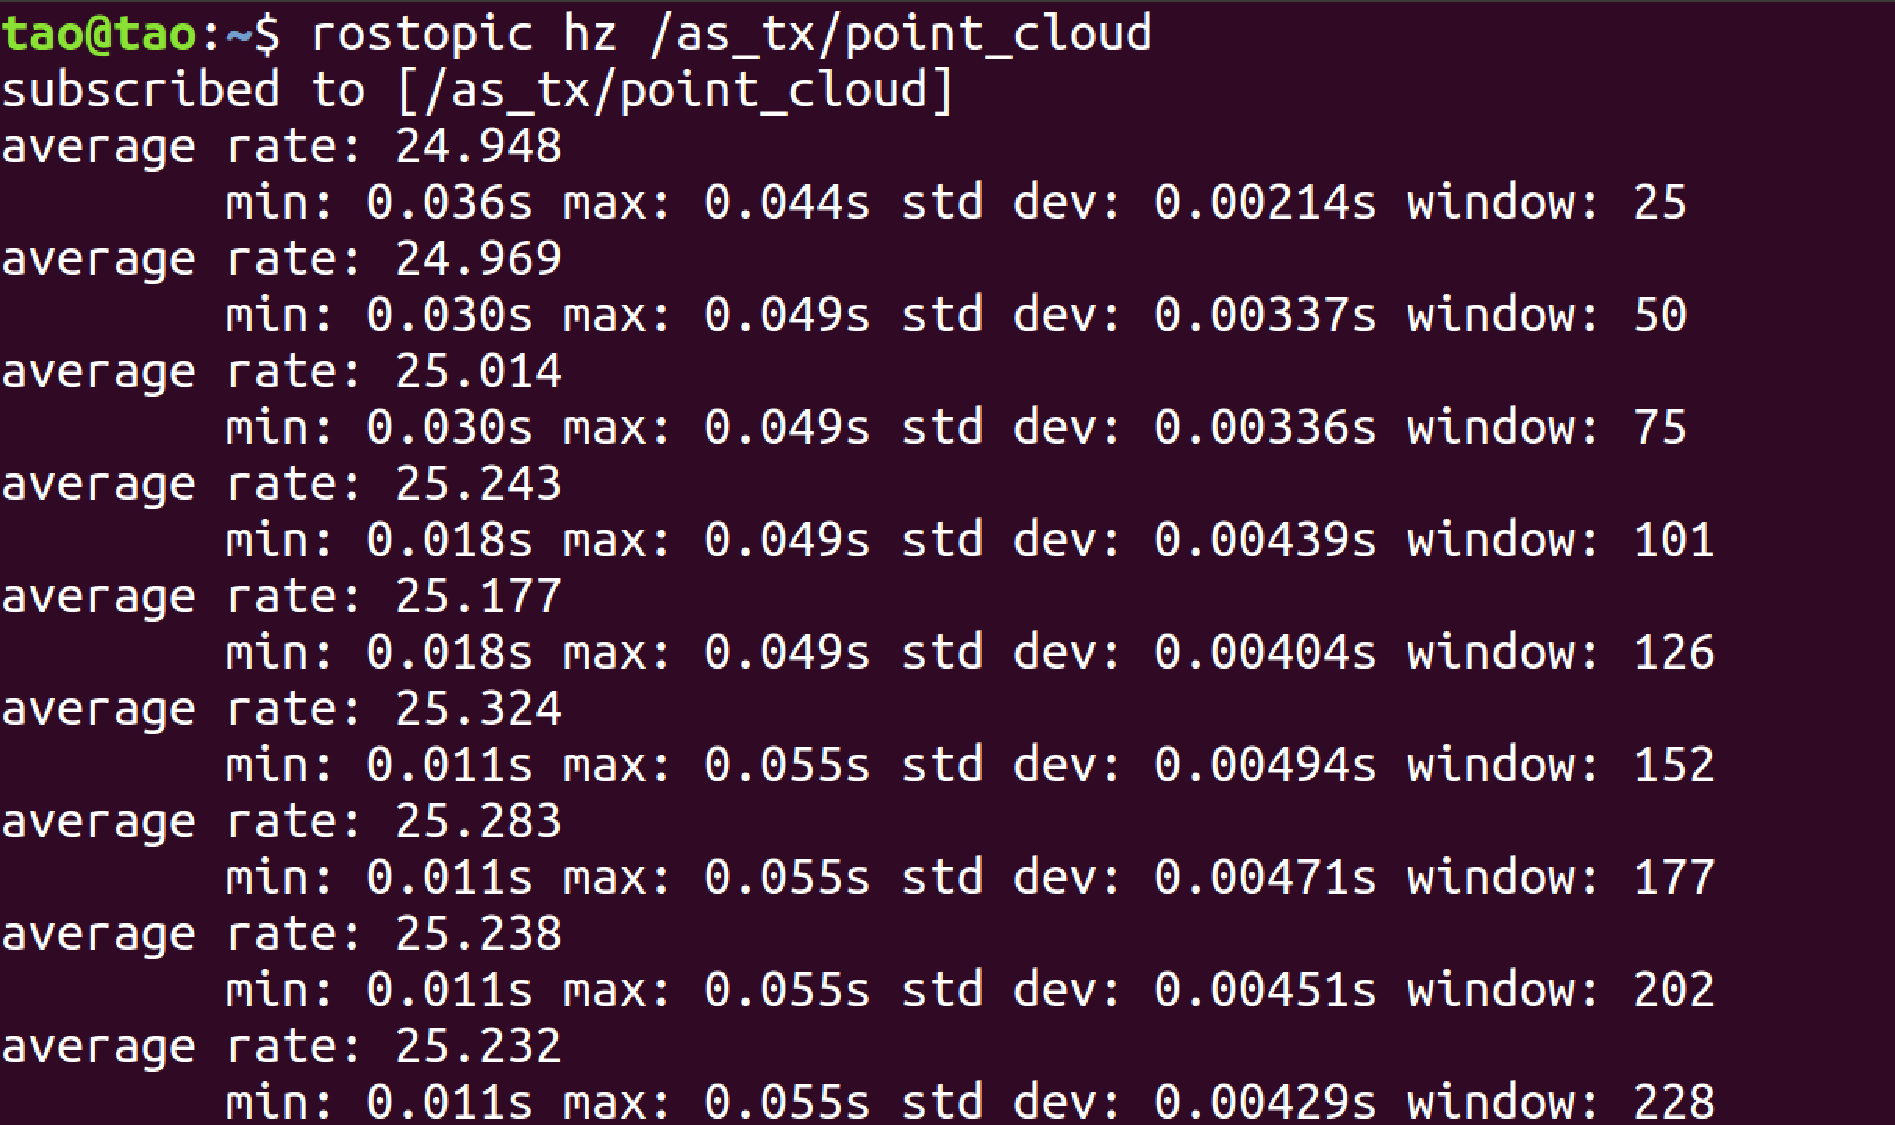
\includegraphics[width=0.8\textwidth]{pics/F_PCL.pdf}
	\caption{Frequenz von Information �ber Punktwolke}
	\label{fig:F_PCL}
\end{figure}
\begin{figure}[htbp] 
	\centering
	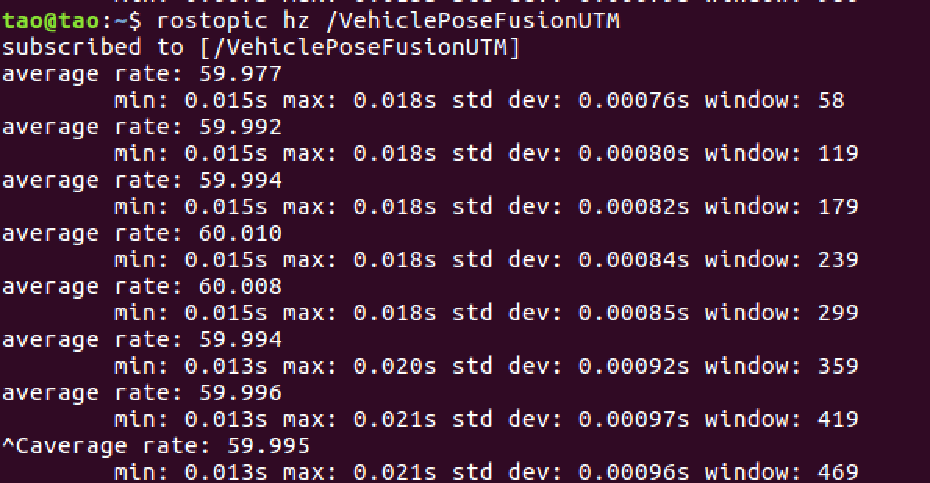
\includegraphics[width=0.8\textwidth]{pics/F_UTM.pdf}
	\caption{Frequenz von Information �ber UTM-Koordinaten}
	\label{fig:F_UTM}
\end{figure}
\begin{figure}[htbp] 
	\centering
	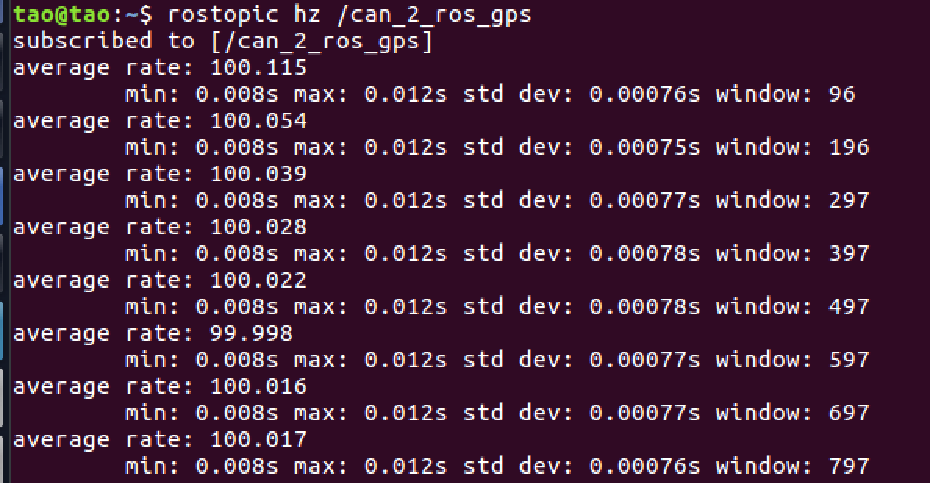
\includegraphics[width=0.9\textwidth]{pics/F_can_gsps.pdf}
	\caption{Frequenz von Information �ber Nickelwinkel}
	\label{fig:F_can_gsps}
\end{figure}
\begin{figure}[htbp] 
	\centering
	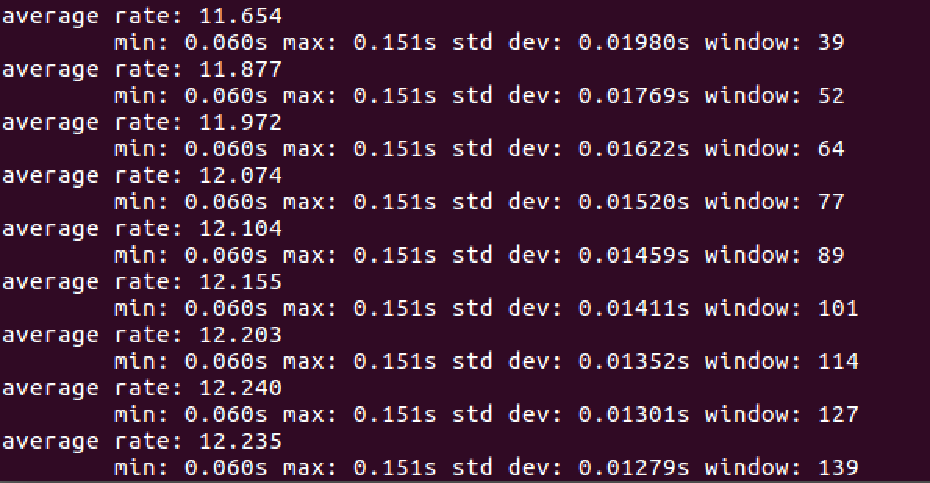
\includegraphics[width=0.9\textwidth]{pics/OUTPUT12Hz.pdf}
	\caption{Frequenz der Modellausgangsdaten}
	\label{fig:OUTPUT12Hz}
\end{figure} 